\section{Results}
\label{sec:results}

We test the four proposed dispatching strategies in the Zurich scenario with ten
runs per fleet size and strategy. Since the dispatchers rely on freeflow speeds in the network
for their routing when the simulation starts, we let each run perform 20 iterations
in which the dispatcher step by step senses the traffic conditions, e.g. how to
avoid traffic jams at peak hours.

The dispatching stages of all algorithms are called once every 60 seconds in
simulated time, while the rebalancing periods for the feedforward and feedback
dispatcher are 10 minutes and 20 minutes, respectively. Those values have been
obtained from prior simulation runs.

For Zurich, the times with peak congestion and, hence, longest travel times
are from 6:30pm to 9:00am and from 4:30pm to 6:30pm. Figure \ref{fig:mean_peak_waiting_times}
shows the average customer wait time over the whole day and just for peak hours.
While the simple heuristic approach consistently yields the longest wait times
for any fleet size, the feedback dispatcher performs best. The bipartite matching
performs in between, since it is based on an optimal request assignment, but does
not do any rebalancing. Surprisingly, the feedforward dispatcher performs similar
to the bipartite matching algorithm. This means, that the expected demand that
has been generated from the scenario data does not optimally predict the actual
travel patterns in the simulation.

Assuming that 5 minutes at peak times are an acceptable wait time, that delay is
achieved with a fleet of 10,000 vehicles for the heuristic, but with only 8,700
for the feedback dispatcher.

\captionsetup[subfigure]{width=0.9\textwidth}

\begin{figure}
    \centering
    \begin{subfigure}[t]{0.495\textwidth}
        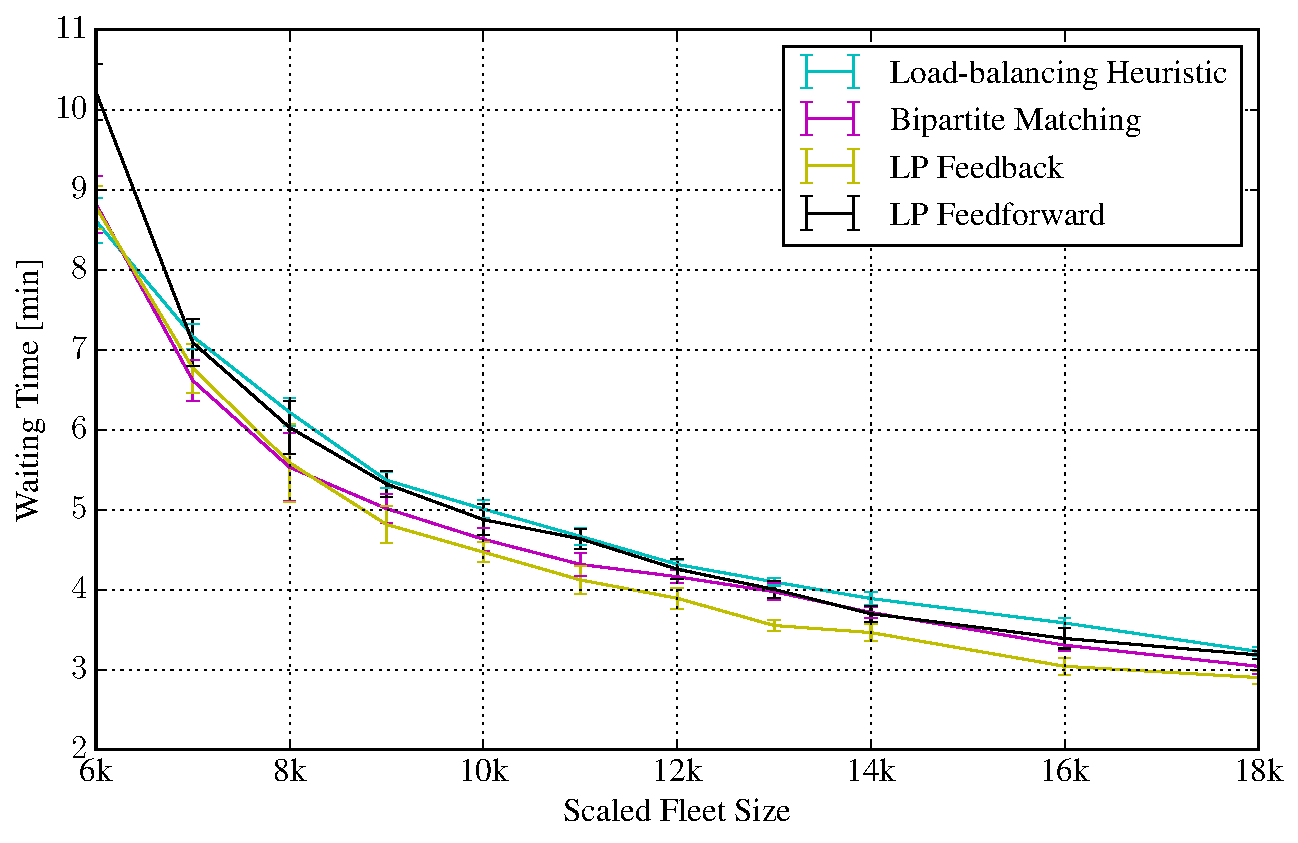
\includegraphics[width=1.0\textwidth]{figures/mean_peak_waiting_times.pdf}
        \caption{Average waiting time for an AV to arrive at peak times (solid) and over the entire day (dashed)}
        \label{fig:mean_peak_waiting_times}
    \end{subfigure}\hfill
    \begin{subfigure}[t]{0.495\textwidth}
        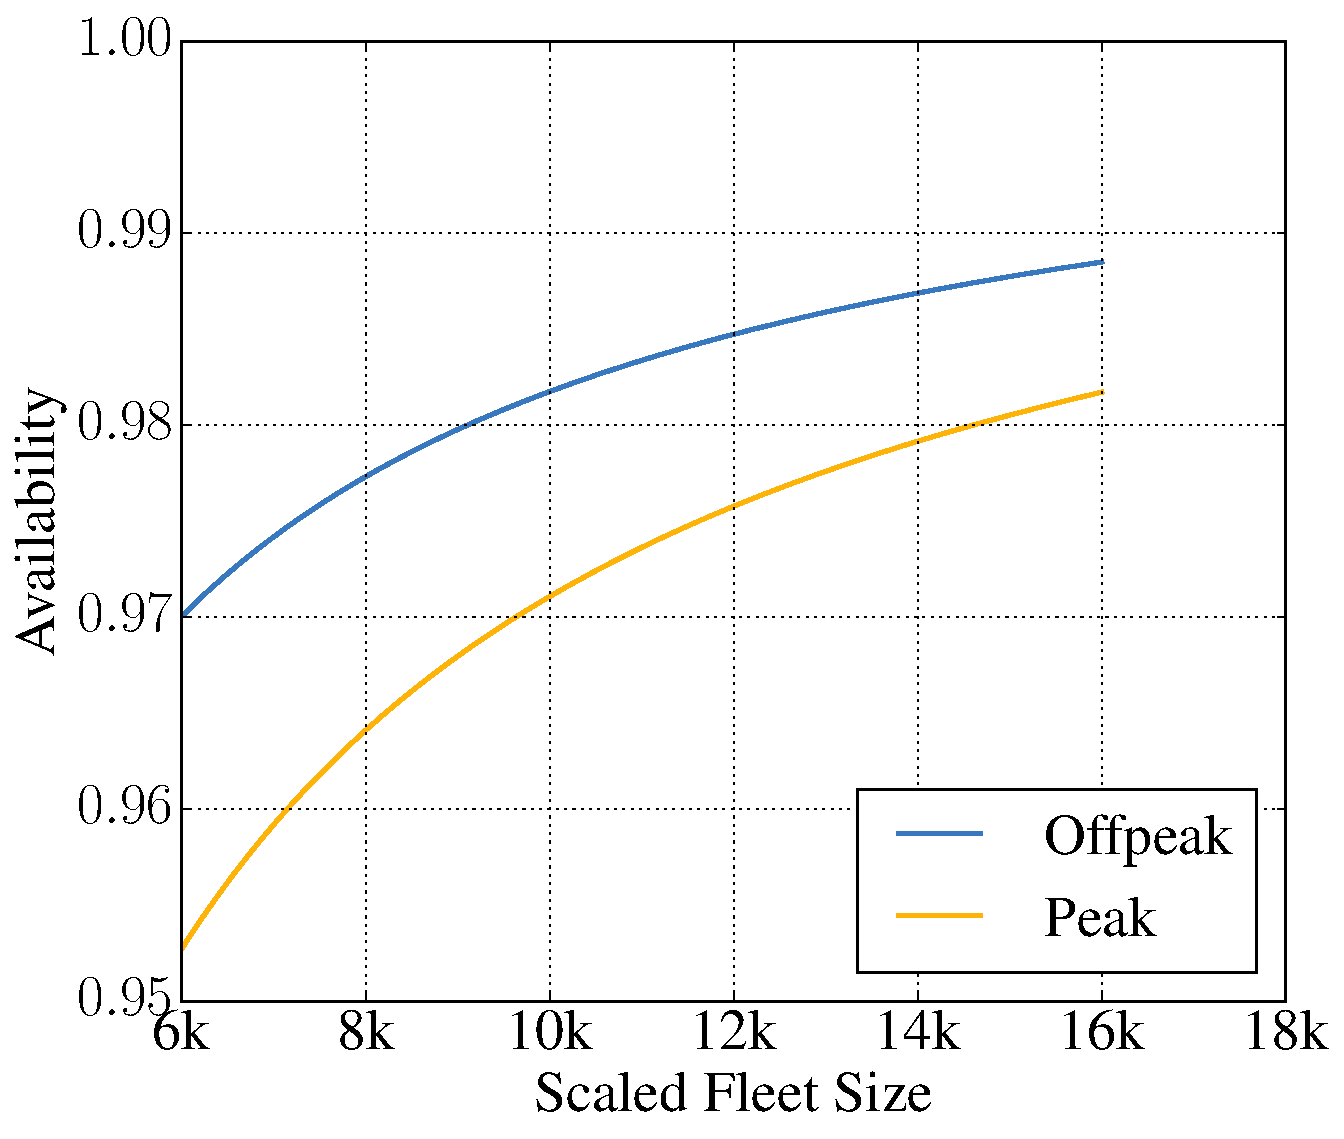
\includegraphics[width=1.0\textwidth]{figures/availability.pdf}
        \caption{Probability of at least one AV being available whenever a request comes in
        TODO: Make same range a waiting time and same scaling}
        \label{fig:performanceavailability}
    \end{subfigure}
    \caption{Fleet performance metrics for different l}
\end{figure}







%\begin{figure}
%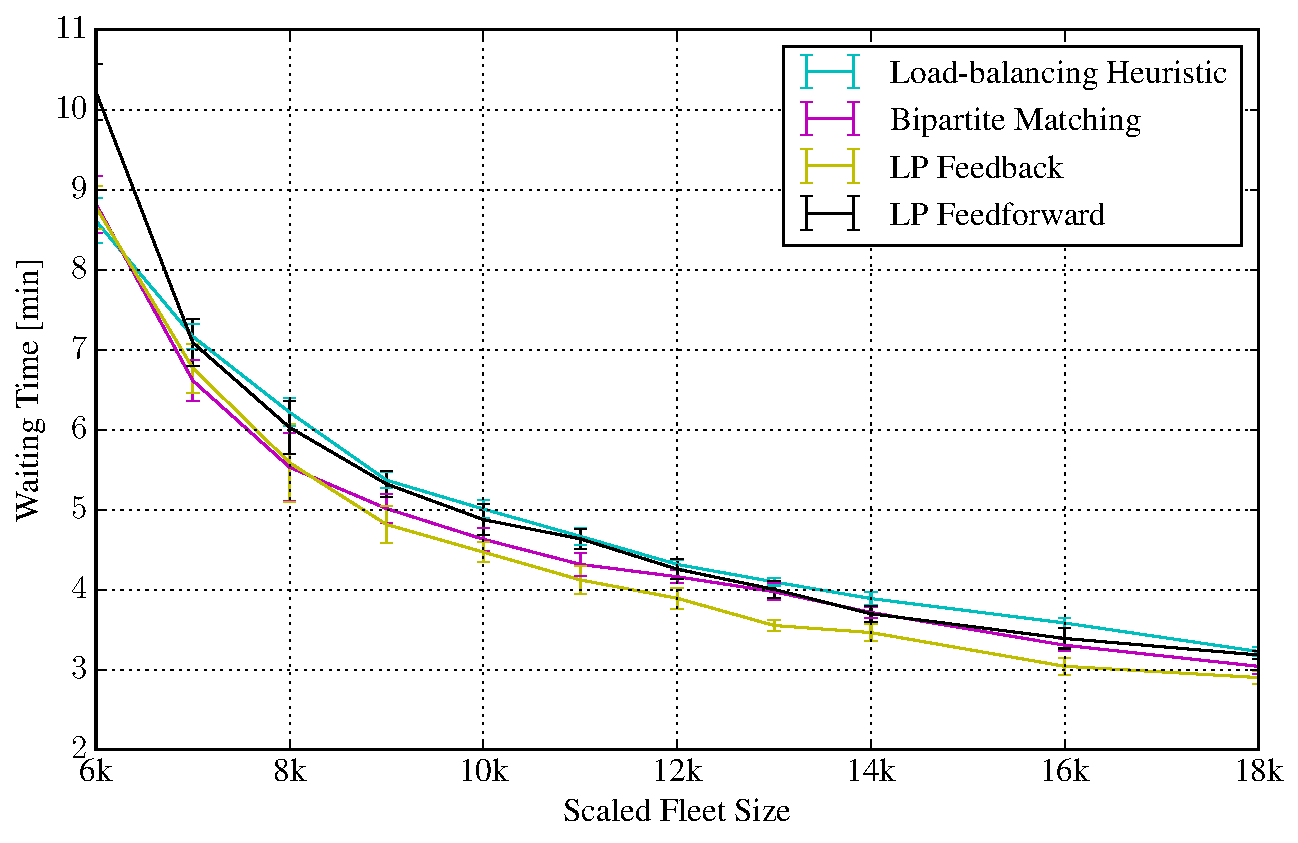
\includegraphics[width=1.0\textwidth]{figures/mean_peak_waiting_times.pdf}
%\caption{Average waiting time for an AV to arrive at peak times (solid) and over the entire day (dashed)}
%\label{fig:mean_peak_waiting_times}
%\end{figure}

[TODO: Updat empty rides!!!]

Figure \ref{fig:empty_rides} shows the percentage of fleet mileage that is driven
without a customer, either for pickup or rebalancing purposes. Clearly, the LP
algorithms, which both use rebalancing, have a higher share of empty mileage
that the non-rebalancing approaches. The heuristic approach manages to keep the
share lowest, since it mainly operates in a best-response state, where only the
shortest pickup trips are chosen. Remarkably, the total driven distance for all
dispatchers is very similar (Figure \ref{fig:total_distance}), which indicates
that the surplus of empty distance for the intelligent dispatchers does not stem
from inefficient movements, but rather effective movements towards the expected
customer demand for shorter waiting times.

[TODO: Do we need two plots here? Also a plot Total Distance <-> Relative Distance
would be possible, where one can traverse the fleet size along the graph]

%\begin{figure}
%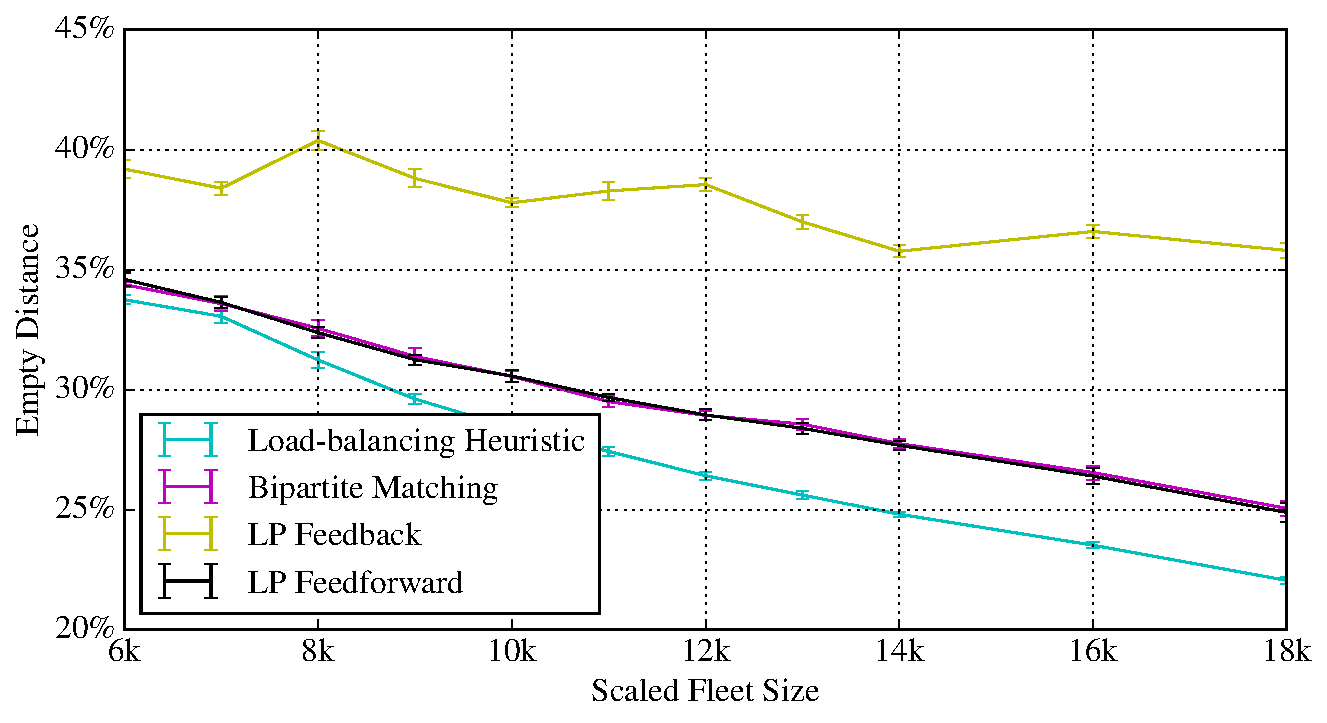
\includegraphics[width=1.0\textwidth]{figures/empty_rides.pdf}
%\caption{The fraction of distance that is driven by AVs without a passenger.}
%\label{fig:empty_rides}
%\end{figure}

%\begin{figure}
%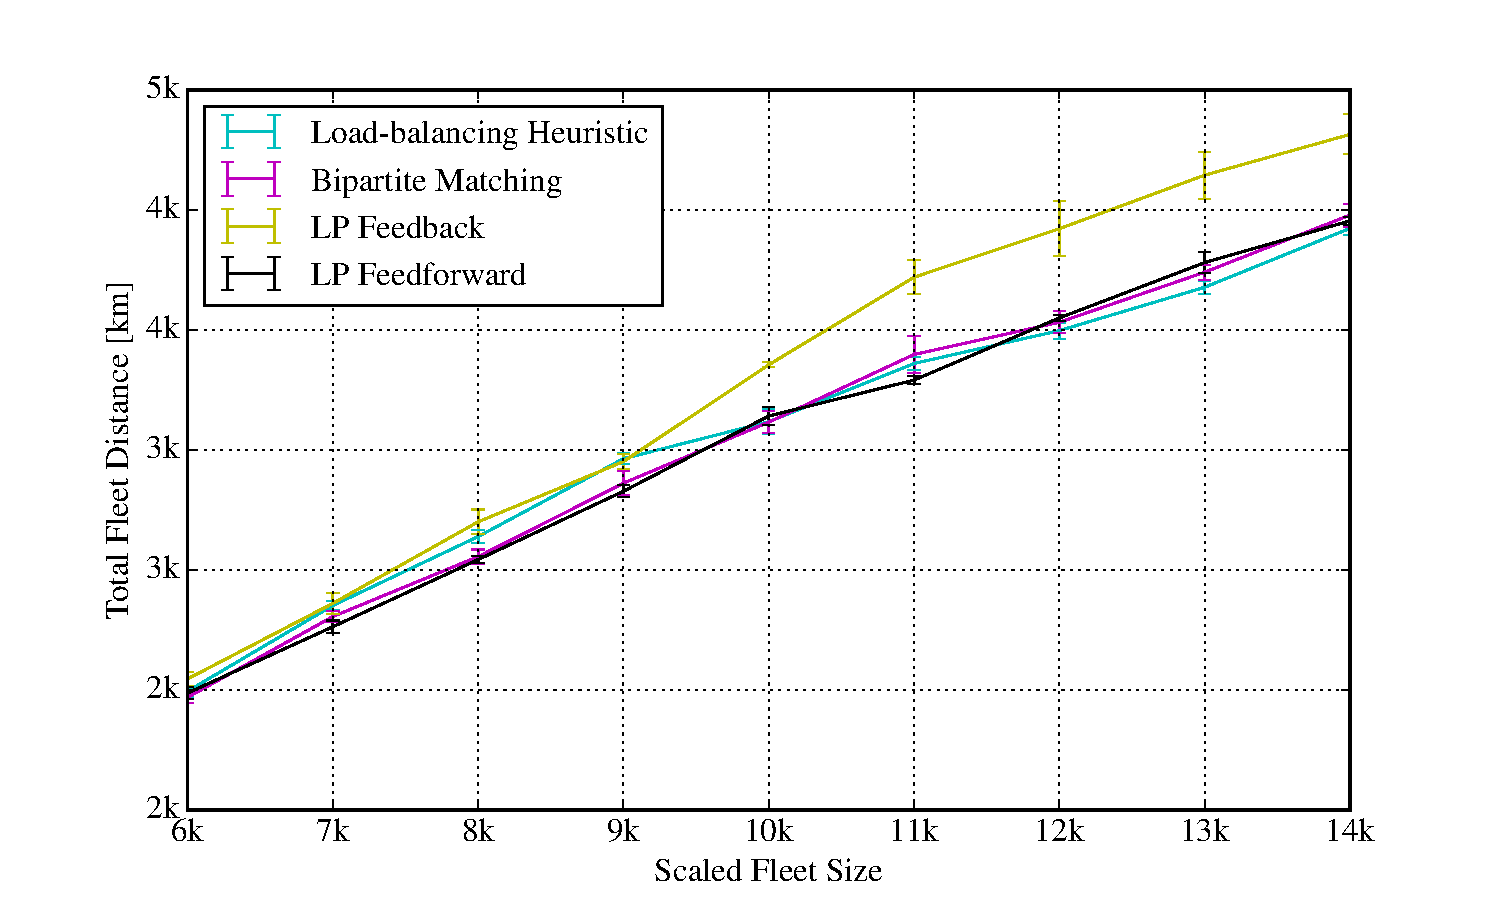
\includegraphics[width=1.0\textwidth]{figures/total_distance.pdf}
%\caption{The total distance that is driven by AVs, with and without passenger on-board.}
%\label{fig:total_distance}
%\end{figure}

\begin{figure}
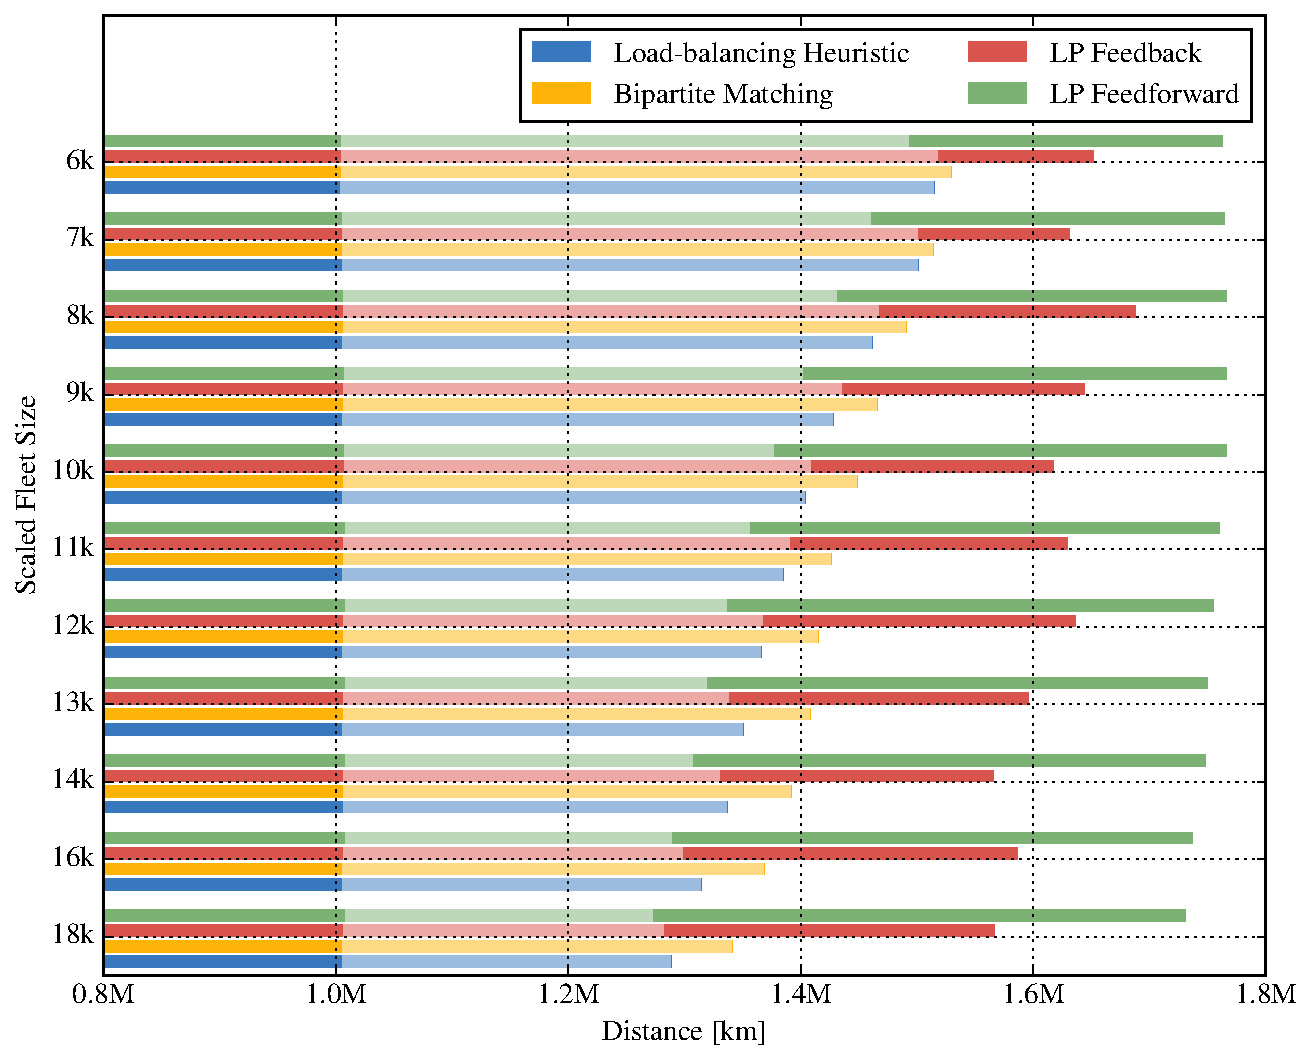
\includegraphics[width=1.0\textwidth]{figures/distances.pdf}
\caption{Distribution of distances for different fleet sizes. From left to right:
Customer distance, empty pickup distance, empty rebalancing distance.}
\label{fig:distances}
\end{figure}

Finally, the occupancy of the fleet is measured. For a fleet size of 6,000
vehicles, they are busy carrying a passenger for around 4.8h per day, while
this value drops to 2.16h for the maximum fleet size of 140,000. In both cases,
those numbers exceed the average 1.92h [TODO Cite, do we have this for switzerland???] of today's vehicle fleet.
Comparing the heuristic and feedback dispatchers at a fleet size for five minute
wait time, the vehicles in the latter one are occupied almost one hour more per day.

\subsection{Cost Analysis}
\label{sec:cost_analysis}

Based on the cost calculator for fleets of automated vehicles by Bösch et al. \cite{cost_paper}
 the costs of operating the simulated
AV services are computed. Specifically, by providing the calculator with key
figures of the operator (among them the occupancy, the share of empty rides, the
average travel distance) the price that the operator would at least need to ask
a customer per kilometer is computed. The calculation
is based on a detailed analysis of running and fixed costs and includes a
profit margin of 3\% for the operator. Figure~\ref{fig:passenger_price}
shows the results from this analysis. Unsurprisingly, the price that needs to be
charged from the customer increases with larger fleet sizes, while a clear difference
between the algorithms can be observed. Clearly, the simple heuristic is the most
costly operating scheme, while the feedback dispatcher can be operated with the
lowest passenger prices.

\begin{figure}
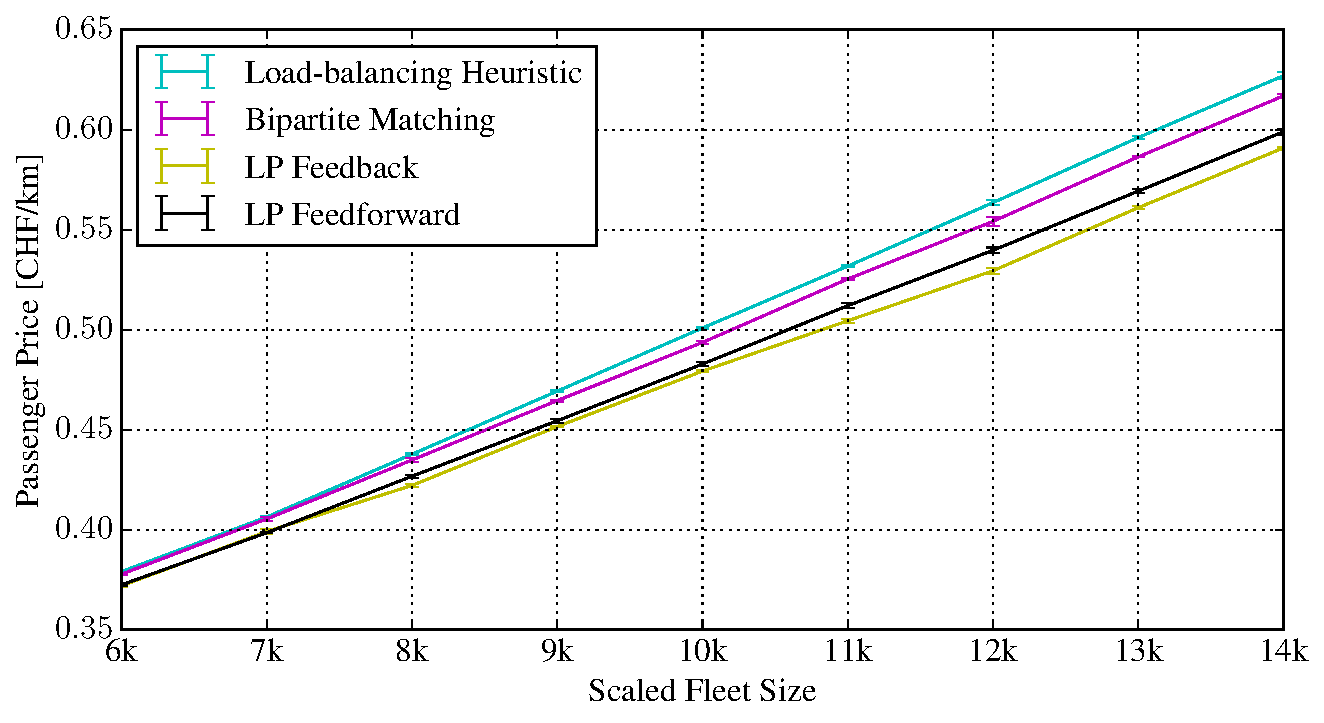
\includegraphics[width=1.0\textwidth]{figures/01_passenger_price.pdf}
\caption{The minimum customer prices that an AV operator needs to charge the customer
in order to have a profit margin of at least 3\%.}
\label{fig:passenger_price}
\end{figure}

Compared to the average price of a taxi operator in Zurich (6 CHF/km, [TODO Cite])
the computed prices are extremely low. Hence, an automated service would clearly
push conventional taxi operators out of the market. While in the short term a
private vehicle today is cheaper than the analysed AV services (0.17 CHF/km, [CITE])
except for very large fleet sizes the service is cheaper in the long run (compared
to 0.72 CHF/km overall costs of owning a private car). However, compared to
(subsidized) prices for public transport (0.25 CHF/km), the services are more
expensive.

Therefore, the proposed AV services are highly attractive to car users, but may
not be able to compete with subsidized public transport. On the other hand, AVs
allow for more direct trips and thus for savings in travel time. Further studies
may analyse how these affect the attractiveness of the AMoD services.

Looking at different choice alternatives for customers, two components are important
that are weighed against each other: The expected wait time and the price. Figure
\ref{fig:time_vs_price} combines the key results from our simulations. There,
the price that a specific operator configuration (fleet size and dispatcher)
needs to charge is
displayed in comparison to the wait time that this operator is offering.
At a wait time of five minutes an operator would be able to offer a satisfactory service
for around 0.45 CHF with the feedback dispatcher, while he would need to charge
0.50 CHF with the simple load-balancing heuristic. 

%The better the level of service of the operator is, the larger this margin becomes.

\begin{figure}
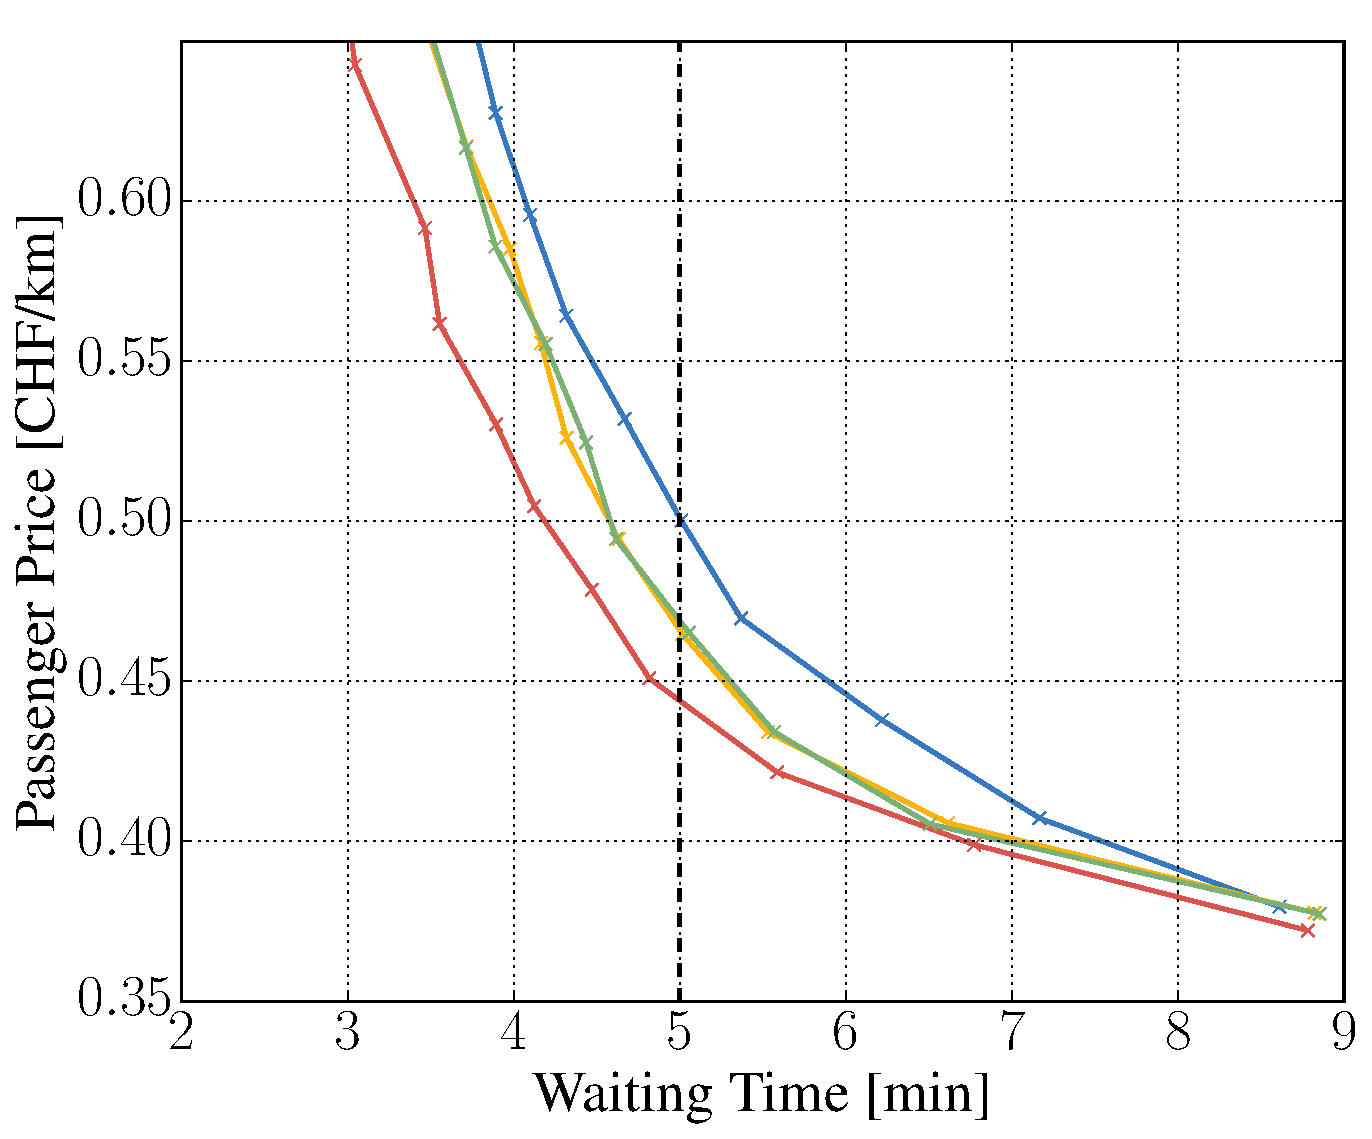
\includegraphics[width=1.0\textwidth]{figures/time_vs_price.pdf}
\caption{Comparison plot of offered wait times and minimum service prices for the
simulated fleet configurations}
\label{fig:time_vs_price}
\end{figure}
